%% Copernicus Publications Manuscript Preparation Template for LaTeX Submissions
%% ---------------------------------
%% This template should be used for copernicus.cls
%% The class file and some style files are bundled in the Copernicus Latex Package, which can be downloaded from the different journal webpages.
%% For further assistance please contact Copernicus Publications at: production@copernicus.org
%% https://publications.copernicus.org/for_authors/manuscript_preparation.html


%% Please use the following documentclass and journal abbreviations for discussion papers and final revised papers.

%% 2-column papers and discussion papers
\documentclass[npg, manuscript]{copernicus}


%% Journal abbreviations (please use the same for discussion papers and final revised papers)


% Advances in Geosciences (adgeo)
% Advances in Radio Science (ars)
% Advances in Science and Research (asr)
% Advances in Statistical Climatology, Meteorology and Oceanography (ascmo)
% Annales Geophysicae (angeo)
% Archives Animal Breeding (aab)
% ASTRA Proceedings (ap)
% Atmospheric Chemistry and Physics (acp)
% Atmospheric Measurement Techniques (amt)
% Biogeosciences (bg)
% Climate of the Past (cp)
% DEUQUA Special Publications (deuquasp)
% Drinking Water Engineering and Science (dwes)
% Earth Surface Dynamics (esurf)
% Earth System Dynamics (esd)
% Earth System Science Data (essd)
% E&G Quaternary Science Journal (egqsj)
% Fossil Record (fr)
% Geographica Helvetica (gh)
% Geoscientific Instrumentation, Methods and Data Systems (gi)
% Geoscientific Model Development (gmd)
% History of Geo- and Space Sciences (hgss)
% Hydrology and Earth System Sciences (hess)
% Journal of Micropalaeontology (jm)
% Journal of Sensors and Sensor Systems (jsss)
% Mechanical Sciences (ms)
% Natural Hazards and Earth System Sciences (nhess)
% Nonlinear Processes in Geophysics (npg)
% Ocean Science (os)
% Primate Biology (pb)
% Proceedings of the International Association of Hydrological Sciences (piahs)
% Scientific Drilling (sd)
% SOIL (soil)
% Solid Earth (se)
% The Cryosphere (tc)
% Web Ecology (we)
% Wind Energy Science (wes)


%% \usepackage commands included in the copernicus.cls:
%\usepackage[german, english]{babel}
%\usepackage{tabularx}
%\usepackage{cancel}
%\usepackage{multirow}
%\usepackage{supertabular}
%\usepackage{algorithmic}
%\usepackage{algorithm}
%\usepackage{amsthm}
%\usepackage{float}
%\usepackage{subfig}
%\usepackage{rotating}
\usepackage{easy-todo}
\usepackage{graphicx}

% À changer
\newcommand{\yobs}{\mathbf{y}^o}
\DeclareMathOperator*{\argmin}{arg\,min \,}
\DeclareMathOperator*{\argmax}{arg\,max \,}
\newcommand{\Var}{\mathbb{V}\textrm{ar}}
\newcommand{\Ex}{\mathbb{E}}
\newcommand{\Prob}{\mathbb{P}}
\newcommand{\Cov}{\textsf{Cov}}
\newcommand{\tra}{\mathrm{tr}}
\newcommand{\kmean}{\hat{\mathbf{k}}_{\mathrm{mean}}}
\newcommand{\checkap}{\check{\alpha}_p}
\newcommand{\checkkp}{\check{\mathbf{k}}_p}
\begin{document}

\title{Titre -- 05/12/2018}%TEXT}


% \Author[affil]{given_name}{surname}

\Author[]{Victor}{Trappler}
\Author[]{Élise}{Arnaud}
\Author[]{Laurent}{Debreu}
\Author[]{Arthur}{Vidard}

\affil[]{Univ. Grenoble Alpes, CNRS, Inria, Grenoble INP*, LJK, 38000 Grenoble, France}
% \affil[]{ADDRESS}

%% The [] brackets identify the author with the corresponding affiliation. 1, 2, 3, etc. should be inserted.



\runningtitle{Title}

\runningauthor{Trappler V.}

\correspondence{Victor Trappler (victor.trappler@univ-grenoble-alpes.fr)}



\received{}
\pubdiscuss{} %% only important for two-stage journals
\revised{}
\accepted{}
\published{}

%% These dates will be inserted by Copernicus Publications during the typesetting process.


\firstpage{1}

\maketitle

% \listoftodos\

\begin{abstract}
Classical methods of parameter estimation usually imply the minimisation of an objective function, that measures the error between some observations and the results obtained by a numerical model. In the presence of random inputs, the objective function becomes a random variable, and notions of robustness have to be introduced.

In this paper, we are going to present how to take into account those uncertainties by defining a notion of robustness based on the distribution of the conditional minimisers and compare it with the minimum in the mean sense, and the minimum of variance.

This will then be applied on a academic problem of robust estimation of bottom friction for a numerical model of the one dimensional shallow water equations.
\end{abstract}

\copyrightstatement{TEXT}

%----------------------------------------------------------------------------
\listoftodos{}


\introduction%% \introduction[modified heading if necessary]
\subsection{Motivation}

The process of modelling a physical phenomenon usually implies to add some errors. These uncertainties come from different mandatory steps, such as the discretisation of the domain, or simplifications to take into account subscale phenomena. These unresolved processes are usually represented by corrective terms involving parametrisation. Once those parameters have been identified, they have to be estimated, so that the numerical model matches as closely as possible the reality. This is done by the minimisation of a cost function.

The uncertainties in the model are twofold: the ``true'' values of the parameters are yet to be evaluated, while some other parameters are fixed but possibly to a wrong value.
A rough distinction between those types of uncertainty can be found in~\cite{walker_defining_2003}:
\begin{itemize}
\item Epistemic uncertainty is the uncertainty coming from a lack of knowledge, and can be reduced. This is the ignorance of the true value of parameter that we aim at calibrating.
\item Aleatoric uncertainty is the uncertainty coming from the inherent variability of the system studied. This is the ``natural'' variability of some environmental variables. 
\end{itemize}

In this paper, the estimation will consist in reducing the epistemic uncertainty, while taking into account the aleatoric uncertainty. This is what we define as robust estimation.


The definition of robustness differs depending of the context in which it is used. Indeed, a definition of the robustness of an estimator is a measure of the sensibility of said estimator to outliers~\citep{huber_robust_2011}. This lead to the introduction of robust norms in data assimilation, such as the Huber norm in~\cite{rao_robust_2015}. The point of this norm is to assume Gaussian distribution for small errors (the usual $L_2$ norm), while the large errors are assumed to be Laplace distributed (so the $L_1$ norm).
In other cases, robustness in a Bayesian framework refers to the sensitivity to a wrong specification of the priors~\citep{berger_overview_1994}.



In our application, the cost function to ``minimise'' is a random variable. We are going to focus on two different notions of robustness: robustness by minimising the mean and variance, as it has been applied to portfolio selection in~\cite{markowitz_portfolio_1952}, and robustness based on the distribution of the minimisers of the function. This information on the location of the minimisers is not a novel idea, as it had been applied as a criterion in sequential Bayesian optimisation \citep{villemonteix_informational_2006,hennig_entropy_2011}. More specifically, the constraint of optimality will be relaxed to define a new estimate.

After having properly defined those robust estimates, an academic problem of estimation of bottom friction will be introduced, and the robust estimates will be computed in Section~\ref{sec:swe_application}.

%\subsection{State of the art}
% \cite{kuczera_there_2010}
% \cite{bect_sequential_2012}


%---------------------------------------------------------------------------


\subsection{Context and notations}

We assume that we have access to a model $\mathcal{G}$, a computer code simulating a physical phenomenon over a specific time window. Different types of parameters for this model can be established \citep{walker_defining_2003}:
\begin{itemize} 
\item A priori chosen parameters, which are chosen, and considered invariant
\item Calibrated parameters, which are unknown and needs to be calibrated.
\end{itemize}
Based on this classification, we define $\mathbf{k}\in \mathcal{K}\subset \mathbb{R}^p$ as the parameter to calibrate, i.e.\ the control variable, while $\mathbf{u}\in\mathcal{U}\subset\mathbb{R}^l$ is a priori chosen, and set at $\mathbf{u}^b$. This parameter represents the environmental conditions of the phenomenon studied.
% In the scope of our application, this parameter is the ocean bed friction induced by its rugosity. The environmental variables are the operating conditions, such as the boundary conditions.
The computer code maps those parameters to an observable physical quantity (such as the sea surface height) that will be compared to an observation $\yobs\in\mathcal{Y}$:

\begin{equation}
  \label{eq:def_M}
  \mathcal{G}: (\mathbf{k},\mathbf{u})\in \mathcal{K}\times\mathcal{U} \longmapsto \mathcal{G}(\mathbf{k},\mathbf{u}) \in \mathcal{Y}
\end{equation}
\section{Calibration: deterministic twin experiments}
\label{sec:deterministic}
% \subsection{Parameter calibration in a deterministic setting}


For the estimation of the ``best'' value of $\mathbf{k}$, we compute first an observation $\yobs$, generated with the couple $(\mathbf{k}^t,\mathbf{u}^t)$, supposed unknown (where ${(\cdot)}^t$ stands for ``truth''):
\begin{equation}
  \yobs = \mathcal{G}(\mathbf{k}^t, \mathbf{u}^t)
\end{equation}
In a data assimilation setting, this calibration consists in the minimisation of the cost function $J$ defined by
\begin{align}
  \label{eq:def_cost_fun}
  J(\mathbf{k}) & = \frac12\|\mathcal{G}(\mathbf{k},\mathbf{u}^b) - \yobs \|_{\mathbf{R}^{-1}}^2 + \mathop{\mathrm{regul}}(\mathbf{k})%\frac12\|\mathbf{k}-\mathbf{k}^b\|_{\mathbf{B}^{-1}}^2
\end{align}
where $\mathop{\mathrm{regul}}$ is a regularisation function taking possibly into account a background value $\mathbf{k}^b$. The matrix $\mathbf{R}$ is the covariance matrix of the observation error. Assuming a well-posed problem, the function $J$ reaches a unique global minimum at $\hat{\mathbf{k}}$:
\begin{equation}
  \label{eq:khat_def}
  \hat{\mathbf{k}} = \argmin_{\mathbf{k} \in \mathcal{K}} J(\mathbf{k})
\end{equation}
This method brings different problems: minimising $J$ will for instance compensate the error introduced by the parametrisation $\mathbf{k}$, but will also compensate another misspecification: choosing $\mathbf{u}^b$ instead of $\mathbf{u}^t$ in the computer code.
In the end, the value $\hat{\mathbf{k}}$ obtained will be optimal for this configuration. However, if the operating conditions do change, there is no information on the performance of $\hat{\mathbf{k}}$ for this other setting. As a result, this may lead to poor results when the calibrated model is used for predictions. This naïve approach is treated in Section~\ref{ssec:deterministic_optimisation}.

Another strategy, minimising $J$ over $\mathcal{K}\times\mathcal{U}$ is not always possible, and not always relevant. The minimisation over the whole joint space may increase the complexity of the problem, and the parameter computed may not be robust in the end. 

The random nature of the environmental variables is treated by introducing a probabilistic framework.
% \begin{figure}[t]
% \includegraphics[width=8.3cm]{Figures/optimization_using_misspecified_uref_4d.pdf}
% \caption{TEXT}
% \end{figure}
% \begin{figure*}[t]
% \includegraphics[width=12cm]{Figures/optimization_using_misspecified_uref_4d.pdf}
% \caption{TEXT}
% \end{figure*}


%----------------------------------------------------------------------------
\section{Stochastic modelling of the cost function}
% \subsection{Probabilistic point of view}
The aleatoric uncertainty on the environmental variables is modelled by a random variable $\mathbf{U}$ whose sample space is $\mathcal{U}$. The probability measure of $\mathbf{U}$ is $\Prob_U$, and its density, if it exists, is $p_U$. Furthermore, $\mathbf{u}^t$ (used to generate $\mathbf{y}^{\mathrm{obs}}$) is sampled from $\mathbf{U}$.
The cost function defined in Eq.~\eqref{eq:def_cost_fun} is no longer a function of solely $\mathbf{k}$, but of $\mathbf{U}$ as well:
\begin{align}
  \label{eq:def_cost_fun_rnd}
  J(\mathbf{k},\mathbf{U}) = \frac12 \| \mathcal{G}(\mathbf{k},\mathbf{U}) - \yobs \|^2_{\mathbf{R}^{-1}} + \mathop{\mathrm{regul}}(\mathbf{k})
\end{align}

For a given $\mathbf{k}$, $J(\mathbf{k},\mathbf{U})$ is a random variable. The main point is to be able to compute a value $\mathbf{k}$ that ``minimises'' in a certain sense the random variable $J(\mathbf{k},\mathbf{U})$.

For a practical purpose, we assume that $\forall \mathbf{u}\in\mathcal{U}$, the minimisation of $\mathbf{k}\mapsto J(\mathbf{k},\mathbf{u})$ is a well-posed problem, and that the minimiser is unique.
Additionaly, the following assumption are made: the cost function is smooth and stricly positive, and $\forall \mathbf{k}\in\mathcal{K}$, the random variable $J(\mathbf{k},\mathbf{U})$ has finite first- and second-order moments.
% ----------------------------------------------------------------------------

\section{Definitions of robustness}
% \todo{Mettre dans intro, plus développer notions de robustesse que je considère pas}
\todoi{Notations $\check{{k}}$/$\hat{k}$ ?}

In this paper, we define robustness as the ability of $\mathbf{k}$ to perform reasonably well under different operating conditions (i.e.\ different $\mathbf{u}$).
In that sense, we introduce two different aspects:
\begin{itemize}
\item Optimisation of the moments of the random variable: usually minimisation of the expected value, or of the variance
  % \begin{itemize}
  % \item Minimise the expected value
  % \item Minimise the variance (or standard-deviation)
  % \item Minimise a function combining mean and variance
  % \end{itemize}
  % \begin{align}
  %   \label{eq:def_opt_mean}
  %   \text{minimise : } \mu(\mathbf{k}) = \Ex_U\left[J(\mathbf{k},\mathbf{U})\right] &= \int_{\mathcal{U}} J(\mathbf{k},\mathbf{u}) \,\mathrm{d}\Prob_U(\mathbf{u})\\
  %                                                                 &= \int_{\mathcal{U}} J(\mathbf{k},\mathbf{u})p_U(\mathbf{u}) \,\mathrm{d}\mathbf{u}
  % \end{align}
  % or
  % \begin{align}
  %   \label{eq:def_opt_var}
  %   \text{minimise : } \sigma^2(\mathbf{k})=\Var_U\left[J(\mathbf{k},\mathbf{U})\right] = \Ex_U\left[\left(J(\mathbf{k},\mathbf{U})-\mu(\mathbf{k})\right)^2\right]
  % \end{align}
\item Study of the distribution of the minimisers, assuming the inverse problem is well-posed to ensure the existence and the unicity of the minimiser for each $\mathbf{u}$. The function of condidtional minimisers is then defined by:
  \begin{equation}
   \mathbf{k}^*: \mathbf{u}\in\mathcal{U} \longmapsto \mathbf{k}^*(\mathbf{u}) = \argmin_{{\mathbf{k}}\in\mathcal{K}} J({\mathbf{k}},\mathbf{u}) \in \mathcal{K}
  \end{equation}
  Using this function, we can define the random variable $\mathbf{K}^*$ as
  \begin{equation}
    \label{eq:def_study_minimisers}
    \mathbf{K}^*= \mathbf{k}^*(\mathbf{U})
  \end{equation}
of generalized probability density function
  \begin{equation}
    \label{eq:def_Kopt_reliability}
    p_{K^*}(\mathbf{k}) \propto \Prob_U\left[\mathbf{k} = \mathbf{k}^*(\mathbf{U})% = \argmin_{\tilde{\mathbf{k}}\in\mathcal{K}}J(\tilde{\mathbf{k}},\mathbf{U})
    \right] = R_1(\mathbf{k})
  \end{equation}

  % \begin{equation}
  %   p_{K^*}(\mathbf{k}) = \int_{\mathcal{U}}p_{K^*}(\mathbf{k} |\mathbf{u})p_U(\mathbf{u})\, \mathrm{d}\mathbf{u} = \int_{\mathcal{U}} 1_{(\mathbf{k} = \mathbf{k}^*(\mathbf{u}))}p_U(\mathbf{u})\, \mathrm{d}\mathbf{u} = \Prob_U\left[\mathbf{k} = \mathbf{k}^*(\mathbf{U}) \right]
  % \end{equation}
%   Moreover, the inequality will be later relaxed by introducing $\alpha \geq 1$:
%   \begin{equation}
%     \label{eq:def_Ralpha}
%     R_{\alpha}(\mathbf{k}) = \Prob_U\left[J(\mathbf{k},\mathbf{U})\leq \alpha \min_{\tilde{\mathbf{k}}} J(\tilde{\mathbf{k}},\mathbf{U}) \right]
%   \end{equation}
\end{itemize}


\subsection{Optimisation of the moments}
Optimising the moments is usually a sound approach, when one aims at optimising in a robust manner. Let us first define $\mu(\mathbf{k})$, and $\sigma^2(\mathbf{k})$, the expected value and the variance of the cost function for a given $\mathbf{k}$ as
\begin{align}
  \label{eq:def_mu}
  \mu(\mathbf{k}) &= \Ex_U\left[J(\mathbf{k},\mathbf{U})\right] = \int_{\mathcal{U}} J(\mathbf{k},\mathbf{u}) \, \mathrm{d}\Prob_U(\mathbf{u}) \\
  \label{eq:def_sigma2}
  \sigma^2(\mathbf{k}) &= \Var_U\left[J(\mathbf{k},\mathbf{U})\right] = \int_{\mathcal{U}} \left(J(\mathbf{k},\mathbf{u}) - \mu(\mathbf{k})\right)^2 \, \mathrm{d}\Prob_U(\mathbf{u}) 
\end{align}
Mean response optimisation leads to the estimate $\kmean$ defined by:
\begin{equation}
  \label{eq:stoch_opt_def_mean}
  \kmean = \argmin_{\mathbf{k}\in\mathcal{K}} \mu(\mathbf{k})
\end{equation}
Minimising the variance, leads to $\hat{\mathbf{k}}_{\mathrm{var}}$:
\begin{equation}
  \label{eq:stoch_opt_def_var}
  \hat{\mathbf{k}}_{\mathrm{var}} = \argmin_{\mathbf{k} \in \mathcal{K}} \sigma^2(\mathbf{k})
\end{equation}


From a user point of view, using $\kmean$ will give good results in the long run, so when a lot of different $\mathbf{u}$ are considered. On the other hand, using $\hat{\mathbf{k}}_{\mathrm{var}}$ will ensure that the output of the cost function will be as constant as possible when $\mathbf{u}$ varies, but without any information on its performance.

For a single $\mathbf{u}$ sampled, Chebyshev's inequality gives an upper bound on the probability of being more than $\lambda>0$ units from the mean.
\begin{equation}
  \label{eq:cheby_ineq}
  \Prob_U\left[|J(\mathbf{k}% _{\mathrm{mean}}
    ,\mathbf{U}) - \mu(\mathbf{k}% _{\mathrm{mean}}
    )|> \lambda\right] \leq \frac{\sigma^2(\mathbf{k}% _{\mathrm{mean}}
    )}{\lambda^2}
\end{equation}
This inequality ties the mean and variance, so it usual to consider mean and variance simultaneously. This multiobjective optimisation problem is usually tackled by computating the Pareto front of $\left(\mu(\mathbf{k}),\sigma^2(\mathbf{k})\right)$~\citep{baudoui_optimisation_2012}. As the multiobjective problem is sometimes hard to solve, alternative strategies based on the minimisation of a scalarized version of the vector of objectives are often considered. Those strategies involve for instance a weighted sum of the objectives~\citep{grodzevich_normalization_2006}, or the minimisation of one of the objectives under constraint on the other, named $\epsilon$-constrained method~\citep[applied for instance in][]{lehman_designing_2004}.



% ----------------------------------------------------------------------------

\subsection{Distribution of the minimisers}
\subsubsection{Most probable estimate}
\todoi{Notation MPE ?}
We are now interested in the distribution of the minimisers of the cost function:
\begin{equation}
  \label{eq:def_R1}
  p_{K^*}(\mathbf{k}) \propto R_1(\mathbf{k}) = \Prob_U\left[J(\mathbf{k},\mathbf{U}) = \min_{\tilde{\mathbf{k}}} J(\tilde{\mathbf{k}},\mathbf{U}) \right] = \Prob_U\left[\mathbf{k}= \mathbf{k}^*(\mathbf{U})\right]
\end{equation}

From this definition, $R_1(\mathbf{k})$ is the probability that $\mathbf{k} \in \mathcal{K}$ is optimal.
To have a first insight on the interest of applying robust estimation, we can compute the information brought by this distribution by means of Shannon's entropy defined by

\begin{equation}
  \label{eq:entropy_def}
  H\left[\mathbf{K}^*\right] 
  = -\int_{\mathcal{K}}  \log\left(\frac{\mathrm{d}\Prob_{K^*}}{\mathrm{d}\lambda} \right) \,\mathrm{d}\Prob_{K^*}
\end{equation}
where $\Prob_{K^*}$ is the image measure of the random variable $\mathbf{K}^*$, and $\lambda$ is a base measure on which we compare $\Prob_{K^*}$.
 The distribution is the most informative if $\mathbf{K}^*$ is equal to a constant $\mathbf{k}$ almost surely (with entropy tending to $-\infty$). On the other hand, the distribution is the least informative if $\mathbf{K}^*$ takes values uniformly spread over $\mathcal{K}$.


From the definition of $R_1$ in Eq.~\eqref{eq:def_R1}, we can define the mode of the distribution of the minimisers (if it exists) as $\hat{\mathbf{k}}_{\mathrm{MPE}}$ (where MPE stands for Most Probable Estimate):
\begin{equation}
  \label{eq:MPE}
  \hat{\mathbf{k}}_{\mathrm{MPE}} = \argmax_{k\in\mathcal{K}} R_1(\mathbf{k}) 
\end{equation}
However, if the value of this maximum is not high, it may not be considered robust: this formulation does not provide information on the performance of the estimator for the configuration where it is not optimal (situation that happens with probability $1-R_1(\hat{\mathbf{k}}_{\mathrm{MPE}})$).

\subsubsection{Relaxation of the constraint}
\label{ssec:relax_constraint}

\todoi{Parler plutôt des quantiles de $\frac{J(\mathbf{k},\mathbf{U})}{J(\mathbf{k}^*(\mathbf{U}),\mathbf{U})}$ ?}
For the MPE, the distribution of the conditional minimisers has been estimated. Instead of only considering the optimal values, we are going to consider optimal values and their ``neighbourhood'' as well.

For that purpose, $\alpha \geq 1$ is introduced to relax the equality constraint of Eq.~\eqref{eq:def_R1}.
In that sense, for a given $\mathbf{u}$, $\mathbf{k}$ is deemed acceptable if $J(\mathbf{k},\mathbf{u}) \leq \alpha J(\mathbf{k}^*(\mathbf{u}), \mathbf{u})$. Taking into account the random nature of $\mathbf{U}$,  $R_\alpha(\mathbf{k})$ is defined as the probability that $\mathbf{k}$ is acceptable:
\begin{equation}
  \label{eq:def_Ralpha}
  R_\alpha(\mathbf{k}) = \Prob_U\left[J(\mathbf{k},\mathbf{U}) \leq 
    \alpha J(\mathbf{k}^*(\mathbf{U}),\mathbf{U}) \right]
\end{equation}
In other words, $R_{\alpha}(\mathbf{k})$ is then the probability that $J(\mathbf{k},\mathbf{U})$ is between 
$J(\mathbf{k}^*(\mathbf{U}),\mathbf{U})$ and 
$\alpha J(\mathbf{k}^*(\mathbf{U}),\mathbf{U})$.

The motivation behind this relaxation is to take into account the local behaviour of the function around the conditional minimisers:
For a given $\mathbf{u}$, if the function $\mathbf{k} \mapsto J(\mathbf{k},\mathbf{u})$ is flat around its minimum $\mathbf{k}^*(\mathbf{u})$, then choosing  $\mathbf{k}^*(\mathbf{u}) + \epsilon$ (for a small $\epsilon$) will produce a value closer to the minimum than when the function has a high curvature.
In addition to that, relaxing the constraint using a multiplicative constant puts more weight (i.e.\ a slower increase of the acceptable region) on the values of $\mathbf{k}^*(\mathbf{u})$ when $J(\mathbf{k}^*(\mathbf{u}),\mathbf{u})$ is close to zero.

Under the assumption that $J>0$, $R_{\alpha}(\mathbf{k})$ is increasing with respect to $\alpha$ for any $\mathbf{k}\in\mathcal{K}$. 
From Eq.~\eqref{eq:def_Ralpha}, we can obtain an upper bound for relevant values of $\alpha$, provided that the maximum and minimum of $J$ is attained on $\mathcal{K}\times\mathcal{U}$:
\begin{equation}
  \label{eq:upper_bound_alpha}
  \alpha \geq \frac{\max_{(\mathbf{k},\mathbf{u})} J(\mathbf{k},\mathbf{u})}{\min_{(\mathbf{k},\mathbf{u})} J(\mathbf{k},\mathbf{u}) } \iff R_\alpha(\mathbf{k}) = 1 \quad \forall \mathbf{k}\in\mathcal{K}
\end{equation}





Let us set a level of confidence $0<p \leq 1$. We are now looking for $\check{\alpha}_p$, the smallest $\alpha$, such that there exists a particular $\checkkp \in \mathcal{K}$ for which $J(\check{\mathbf{k}}_p,\mathbf{U}) \leq \check{\alpha}_p J(\mathbf{k}^*(\mathbf{U}), \mathbf{U})$ with probability $p$. As $R_\alpha$ is increasing with respect to $\alpha$,  $\check{\alpha}_p$ can then be defined as
\begin{equation}
  \label{eq:def_alpha_check}
  \checkap = \inf_{\alpha\geq 1} \left\{ \alpha \mid \exists \checkkp \in \mathcal{K},\, R_{\alpha}(\checkkp) \geq p \right\}
\end{equation}

In other words, this definition can be seen as the construction of the smallest confidence interval of level $p$:
\begin{equation}
  \label{eq:def_CI}
  \Prob_U\left[ \frac{J(\checkkp,\mathbf{U})}{J(\mathbf{k}^*(\mathbf{U}),\mathbf{U})}\in [1, \alpha_p]\right] = p
\end{equation}

By considering the particular case of $\check{\alpha}_1$ a relation between $\check{\mathbf{k}}_1$ and $\check{\alpha}_1$ can be derived:
\begin{equation}
  \label{eq:upper_bound_alpha_check}
  \check{\alpha}_1 = \sup_{\mathbf{u}\in\mathcal{U}} \left\{\frac{J(\check{\mathbf{k}}_1,\mathbf{u})}{J(\mathbf{k}^*(\mathbf{u}), \mathbf{u})} \right\} 
\end{equation}
A high value of $\check{\alpha}_1$ corresponds to a high variability of the response of the function for at least one particular $\mathbf{u}$. In that sense, $J(\check{\mathbf{k}}_1,\mathbf{u})$ may be possibly very high.
For this reason, it is important to study jointly $\checkap$ and $\checkkp$, as the value of $\checkap$ is an information on the ``robustness'' of the solution as it is linked to the range of $\mathbf{u}\mapsto J(\check{\mathbf{k}}_p,\mathbf{u})$.
The different estimators introduced in this paper are summarised in Table~\ref{tab:RO_recap}.

\begin{table*}[!h]
  \caption{Robust estimators, based on a cost function $J$}
  \label{tab:RO_recap}
\begin{tabular}{rlr}
  \tophline
  Estimate & Definition & Interpretation \\
  \middlehline
  $\hat{\mathbf{k}}_{\mathrm{mean}}$ & $\argmin_{\mathbf{k}\in\mathcal{K}} \Ex_U\left[J(\mathbf{k},\mathbf{U})\right]$& Long run performances\\
  $\hat{\mathbf{k}}_{\mathrm{var}}$ & $\argmin_{\mathbf{k}\in\mathcal{K}} \Var_U\left[J(\mathbf{k},\mathbf{U})\right]$ & Steady performances\\
  $\hat{\mathbf{k}}_{\mathrm{MPE}}$ & $\argmax_{\mathbf{k}\in\mathcal{K}} \Prob_U\left[\mathbf{k} = \mathbf{k}^*(\mathbf{U})\right]$& Most often minimiser\\
  $(\check{\mathbf{k}}_{p},\check{\alpha}_p)$ &  $\inf_{\alpha\geq 1} \left\{ \alpha \mid \exists \checkkp \in \mathcal{K},\, R_{\alpha}(\checkkp) \geq p \right\} $& Acceptable values with fixed probability $p$ \\
  \bottomhline
\end{tabular}
\end{table*}


\subsection{Illustration}
We are going to study the problem of robust optimisation on a toy problem, based on Branin-Hoo's function defined on $\mathcal{K}=\mathcal{U} = [0, 5]$. This function has been slightly modified to ensure strict positivity.

\begin{align}
  \label{eq:branin_hoo}
 & J_{\mathrm{BH}}(x_1,x_2) = \frac{1}{51.95}\left[\left(\bar{x}_2 - \frac{5.1 \bar{x}_1^2}{4\pi^2} + \frac{5\bar{x}_1}{\pi} -6 \right)^2 + \left(10 - \frac{10}{8\pi}\right)\cos(\bar{x}_1)-44.81\right]+2\\
&  \text{with } \bar{x}_1 = 3x_1-5,\quad \bar{x}_2 = 3x_2
\end{align}

From the function in Eq.~\eqref{eq:branin_hoo}, we define the BH function as $(\mathbf{k},\mathbf{u}) \mapsto J_{\mathrm{BH}}(\mathbf{k},\mathbf{u})$, and BHs as $(\mathbf{k},\mathbf{u}) \mapsto J_{\mathrm{BH}}(\mathbf{u},\mathbf{k})$. Although the functions are quite similar, the asymmetric roles of $\mathbf{k}$ and $\mathbf{u}$  result in different behaviour for the different estimations.
Finally, we assume that $\mathbf{U}\sim \mathrm{Unif}([0;5])$
\subsubsection{Moments and conditional minimisers}

To compute the MPE, we used different methods to estimate the distribution of the minimisers: KDE (kernel density estimation)~\citep{parzen_estimation_1962,bishop_pattern_2006} and the EM algorithm~\citep{dempster_maximum_1977,borman_expectation_2004} to fit a mixture of three Gaussian distributions. Figure~\ref{fig:contours} shows the contour plot, conditional mean and conditional minimisers of the BH function (right) and the BHs function (left).

For the BHs function, we can observe that those two methods give the same results, as the MPE can be estimated at approximately $0.8$. However for the BH function, this gives different results. Using KDE, the MPE is found to be at around $1.5$, while using EM, the MPE is $3.8$. This difference is explained by the accumulation of minimisers at $3.8$: the EM algorithm fits this accumulation with a normal distribution with a very small variance. In the meantime, we can consider the mixing coefficients: the Gaussian centered at $1.5$ has been attributed a weight of $0.608$, while the one centered at $3.8$ has a mixing weight of $0.226$. Ultimately, an optimiser would be more likely to be close to $1.5$, but we do not have information on its performance in this region around this value.



\begin{figure*}
  \includegraphics[width=12cm]{Figures/branin_side_66.pdf}
  \caption{Top Left: BH function along with conditional minimisers in red. Bottom left: Estimated density using KDE and EM algorithm and conditional mean. Right: Same quantities with BHs}
\label{fig:contours}
\end{figure*}



\subsubsection{Relaxation of the constraint}

Following its definition in Eq.~\eqref{eq:upper_bound_alpha_check}, $\check{\alpha}_1$ has been numerically evaluated at $1.9506$ for the BH function. Figure~\ref{fig:contour_alpha} shows the contour plot, and the frontier corresponding to the couples of points $(\mathbf{k},\mathbf{u})$ such that $J(\mathbf{k},\mathbf{u}) = \check{\alpha}_1 J(\mathbf{k}^*(\mathbf{u}), \mathbf{u})$, and the curve $\mathbf{k}\mapsto R_{\check{\alpha}_1}(\mathbf{k})$.
\begin{figure*}[t]
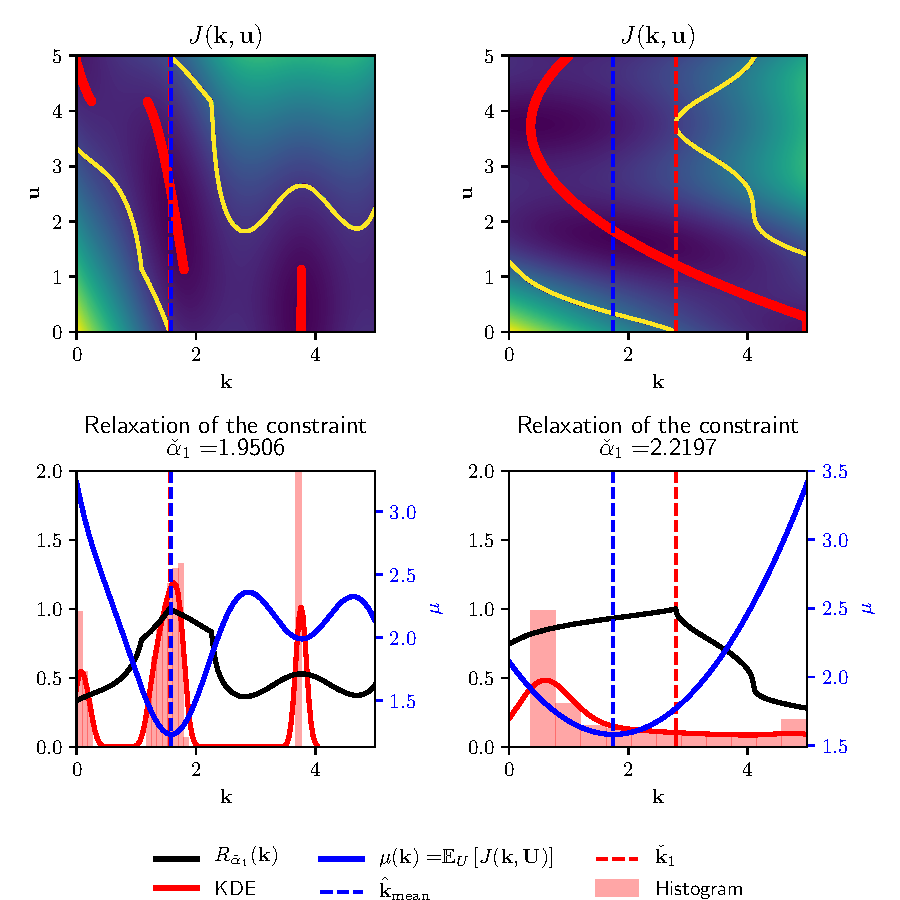
\includegraphics[width=12cm]{Figures/branin_side_66_check.pdf}
\caption{Top: BH function and its conditional minimisers. The thick yellow lines the boundary of the acceptable region, where $\phi_\alpha=0$. The red dashed line is the estimate $\check{k}_{1}$. Bottom: $R_{\check{\alpha}}$, conditional mean and estimated density of the minimisers}
\label{fig:contour_alpha}
\end{figure*}
In Figure~\ref{fig:profiles_branin}, the profiles refers to the function $\mathbf{u}\mapsto J(\mathbf{k},\mathbf{u})$ for a given $\mathbf{k}$, and is useful to visualise the range of values taken by the cost function for different estimates: $\kmean$ minimising the mean value, $\hat{\mathbf{k}}_{\mathrm{var}}$ minimising the variance and $\check{\mathbf{k}}_1$ as defined above. The shaded regions correspond to the interval~$[J(\mathbf{k}^*(\mathbf{u}), \mathbf{u}), \check{\alpha}_1 J(\mathbf{k}^*(\mathbf{u}), \mathbf{u})]$. For this particular problem, the minimiser of the mean response and $\check{\mathbf{k}}_1$ are very close. 

\begin{figure*}[t]
\includegraphics[width=12cm]{Figures/profile_branin.pdf}
\caption{Profiles of BH function for different estimates of $\mathbf{k}$}
\label{fig:profiles_branin}
\end{figure*}


The fact that $\hat{\mathbf{k}}_{\mathrm{mean}}$ and $\check{\mathbf{k}}_1$ are similar is specific to the BH function:
For the BHs function, the two estimates are quite different, as seen on Figure~\ref{fig:contour_alpha}.

The profiles shown Figure~\ref{fig:profiles_branin_switch} explain this difference. In this case $\hat{\mathbf{k}}_{\mathrm{mean}}$ performs very well for $\mathbf{u}>2$, yet for $\mathbf{u}<2$, it produces high values of the function. In that case, performances of $\check{\mathbf{k}}_1$ are closer to the performances of $\hat{\mathbf{k}}_{\mathrm{var}}$, but performs worse than $\hat{\mathbf{k}}_{\mathrm{mean}}$ and $\hat{\mathbf{k}}_{\mathrm{var}}$ for $\mathbf{u}>2$.

\begin{figure*}[t]
\includegraphics[width=12cm]{Figures/profile_branin_switch.pdf}
\caption{Profiles of BHs for different estimates of $\mathbf{k}$}
\label{fig:profiles_branin_switch}
\end{figure*}
% ----------------------------------------------------------------------------
% ----------------------------------------------------------------------------
\clearpage
\section{Application: calibration of a numerical model}
\label{sec:swe_application}
\subsection{Context: Shallow water equations and bottom friction}

The quality of water circulation modelling in coastal areas is largely dependent on the boundary conditions, (e.g.\ the tide), the bathymetry and the friction induced by the rugosity of the ocean bed \citep{boutet_estimation_2015}. The latter will then be estimated in a robust manner, by applying the criteria introduced above.


The model studied is based on the one-dimensional shallow water equations, described Eq.~\eqref{eq:SWE_equations}, solved numerically on a domain $D$. $h$ is the height of the water column, $q$ is the discharge, and $z$ is the bathymetry, while $g$ is the usual gravitation constant. $\mathbf{k}$ is a quadratic friction term, proportional to the square of the inverse of Manning-Strickler coefficient.
\begin{align}
  \label{eq:SWE_equations}
  \left\{
    \begin{array}{l}
      \partial_t h + \partial_x q = 0 \\
      \partial_t q + \partial_x \left(\frac{q^2}{h} + \frac{g}{2}h^2\right) = - gh\partial_x z - \mathbf{k}q |q|h^{-7/3} \\
      h(0, t) = 20.0 + \mathrm{Amplitude} \cdot \sin \left(\frac{2\pi}{\mathbf{u}}t\right) \\
      q(0, t) = 0
      \end{array}
  \right.
\end{align}

The estimation of the bottom friction and/or topography has been treated in a deterministic setting, % in Section~\ref{sec:deterministic}
using tools from variational data assimilation~\cite[e.g.][]{das_estimation_1991,das_variational_1992,honnorat_identification_2010}.
If the boundary conditions are not well-known, the estimation will then compensate this misspecification. The resulting estimate will then be optimal for this particular configuration, but will not acknowledge the uncertainty upon the boundary conditions. Instead, we are looking for an estimate that is robust considering the variability of the uncertain boundary conditions.


The problem of the estimation of the bottom friction will be studied using twin experiments. For this purpose, a few references simulations have been performed in order to produce different observations $\mathbf{y}^o$. Those scenarios are detailed Table~\ref{tab:optim_scenar}. The true bottom fricton $\mathbf{k}^t$ is the same for all simulations, and is a non-constant function of the spatial domain $D = [0, L]$ defined as:
\begin{equation}
  \label{eq:defnitio_kt}
  \mathbf{k}_t= \mathbf{k}_t(x) = 0.2\cdot (1 + \sin(2\pi x/L))
\end{equation}
However, the space $\mathcal{K}$ in which we wish to estimate the bottom friction is one-dimensional. This leads to the strict positivity of the cost function, as no perfect fit can be achieved.

As presented on Table~\ref{tab:RO_modelling}, we consider two a priori chosen variable: $\mathbf{u} \in \mathcal{U}$ that is the period of the sine wave on the left boundary. The aleatoric uncertainty on this variable is modelled by a random variable distributed uniformly on $\mathcal{U}$.
The amplitude of the sine wave is also chosen a priori and set to an arbitrary value, that may be different from the true amplitude used to generate $\mathbf{y}^o$. 



\begin{table*}[!h]
  \caption{Modelling of the estimation problem}
  \label{tab:RO_modelling}
\begin{tabular}{rrr}
  \tophline
  Parameter & Modelling & Type of parameter \\
  \middlehline
  Bottom friction: $\mathbf{k}$  &$\mathcal{K}=[0, 1]$ & Calibrated parameter \\
  Period: $\mathbf{U}$ & $\mathrm{Unif}\left([14.7, 15.3]\right)$ & A priori chosen and uncertain\\
  Amplitude &  5.0 & A priori chosen and fixed\\
  \bottomhline
\end{tabular}
\end{table*}

\subsection{Deterministic optimisation}
\label{ssec:deterministic_optimisation}
The problem has first been studied in a deterministic setting. The following optimisation problem has been performed numerically:
\begin{equation}
  \label{eq:opt_deter}
  \text{Minimise } \mathbf{k}\in\mathcal{K} \mapsto J(\mathbf{k},\mathbf{u}^b)\quad \text{for }\mathbf{u}^b= \Ex_U[\mathbf{U}] = 15.0
\end{equation}
At the same time, the background value of the amplitude is fixed and set to $5.0$.
Different scenario have been established (i.e.\ different $\mathbf{u}^t$ and amplitude producing different $\mathbf{y}^o$), and are detailed in Table~\ref{tab:optim_scenar}. The configurations correspond to different values of the amplitude (letter~``A'') and the period (letter~``P''). If the truth value is greater (resp.\ smaller) than the background value, the lowercase letter ``p'' follows (resp.\ ``m'').

On the same table, are shown the result $\hat{\mathbf{k}}$ of the optimisation defined in Eq.~\eqref{eq:opt_deter} for each one of the different operating conditions.


\begin{table*}[!h]
  \caption{Settings for reference simulations, and optimisation results}
  \label{tab:optim_scenar}
\begin{tabular}{rrrrrrrr} \tophline
Scenario for $\mathbf{u}^t$: &$\Ex_U[\mathbf{U}]$  & Pm & ApPm & AmPm & Pp & ApPp & AmPp \\ \middlehline
  $\mathbf{u}^t- \mathbf{u}^b$ & 0.0            & -0.1  & -0.2 & -0.1 & +0.2 & +0.1 & +0.2 \\
  $\mathrm{Amplitude}- 5.0$   & 0.0             &  0.0  & +0.1 & -0.2 &  0.0 & +0.2 & -0.1 \\ \middlehline
  $\hat{\mathbf{k}}$      & 0.1043          & 0.2028 & 0.2709 & 0.2427 & 0.0  & 0.0 & 0.0015 \\\bottomhline
\end{tabular}
\end{table*}

\begin{table*}[!h]
  \caption{Estimate computed numerically on the Lorenz-63 model}
  \begin{tabular}{*{2}{r}}\tophline
    Estimate & Value \\
    \middlehline
    $\kmean$       & $ 0.008779$ \\
    $\kvar$        & $-0.025338$ \\
    $\kmpe$        & $ 0.008779$ \\
    $\checkk_{0.9}$ & $ 0.008729$ \\
    $\checkk_{0.95}$& $ 0.006078$ \\
    $\checkk_{1}$ &  $ 0.000275$ \\
    \bottomhline
    \end{tabular}
\end{table*}

Optimising without uncertainties (meaning that the $\mathbf{u}^b=\mathbf{u}^t$) yields an optimal value $\hat{\mathbf{k}}$ close to $0.10$, that we define to be $\hat{\mathbf{k}}_{\mathrm{opt}}$
We can observe two different regimes, depending on the sign of $\mathbf{u}^t-\Ex_U[\mathbf{U}]$. If this quantity is positive, optimisation will produce an estimation close to $0$. If it is negative, the estimate is larger than $0.20$.
\subsection{Robust estimates}
In order to compute the robust estimates, the cost function has been evaluated on a regular grid of $150\times150$ points over $\mathcal{K}\times\mathcal{U}$. $\hat{\mathbf{k}}_{\mathrm{mean}}$, $\hat{\mathbf{k}}_{\mathrm{var}}$, $\check{\mathbf{k}}_{.9}$, $\check{\mathbf{k}}_{.95}$ and $\check{\mathbf{k}}_{1}$ (along with their corresponding factors $\check{\alpha}_p$) have been evaluated for the different configurations, detailed in Table~\ref{tab:optim_scenar}. As shown on Table~\ref{tab:res_robust}, $\check{\mathbf{k}}_p$ does not vary significantly when the level of confidence $p$ increases.

\begin{table*}[!h]
  \caption{Mean and variance optimisers, and $\check{\mathbf{k}}_p$ for different levels of confidence $p$}
  \label{tab:res_robust}
  \begin{tabular}{rrrrrrrr} \tophline
    Scenario&$\Ex_U[\mathbf{U}]$ & Pm & ApPm & AmPm & Pp & ApPp & AmPp \\  \middlehline
  $\hat{\mathbf{k}}_{\mathrm{mean}}$ & 0.1678    & 0.2214  & 0.2617 & 0.2685 & 0.0872 & 0.0738 & 0.1275 \\
  $\hat{\mathbf{k}}_{\mathrm{var}}$  & 1.0      &  1.0  & 1.0 & 1.0 &  1.0 & 1.0 & 1.0 \\ \middlehline
  $\check{\mathbf{k}}_{.90}$ & 0.1074 & 0.1074 & 0.0872 & 0.1678 & 0.1074  & 0.0738 & 0.1275 \\
  $\check{\alpha}_{.90}$    & 1.1754  & 1.1718 & 1.1779 & 1.1293 & 1.1768  & 1.1807 & 1.1406 \\\middlehline

  $\check{\mathbf{k}}_{.95}$ & 0.1074 & 0.1074 & 0.0872 & 0.1611 & 0.1074  & 0.0671 & 0.1275 \\
  $\check{\alpha}_{.95}$ & 1.1802 & 1.1806 & 1.1868 & 1.1320 & 1.1861  & 1.2027 & 1.1525 \\\middlehline
    $\check{\mathbf{k}}_{1}$& 0.1074 & 0.1074 & 0.0872 & 0.1611 & 0.1074  & 0.0671 & 0.1275 \\
  $\check{\alpha}_{1}$ & 1.1944    & 1.1922 & 1.1961 & 1.1321 & 1.1976  & 1.2035 & 1.1682 \\\middlehline
\end{tabular}
\end{table*}


In that case, the minimiser of the variance $\hat{\mathbf{k}}_{\mathrm{var}}$ is the right boundary of $\mathcal{K}$, regardless of the value of $\mathbf{u}^t$. This is due to the fact that at this point, the cost function produces bad, yet steady performances. From a physical point of view, increasing the bottom friction will decrease the momentum. The movement of the water surface will be damped, and the operating conditions will have less effects.


Looking at $\hat{\mathbf{k}}_{\mathrm{mean}}$, we can see that the estimates obtained are larger than $0.22$ when $\mathbf{u}^t< \Ex_U[\mathbf{U}]$ (that is for Pm, ApPm, and AmPm). Those results are similar to the one obtained in the deterministic setting of Table~\ref{tab:optim_scenar}. However, for $\mathbf{u}^t> \Ex_U[\mathbf{U}]$ (Pp, ApPp, and AmPp), $\hat{\mathbf{k}}_{\mathrm{mean}}$ is much closer to $\hat{\mathbf{k}}_{\mathrm{opt}}$, the optimal value without uncertainties.

Now for $\check{\mathbf{k}}_1$, while the estimates for scenarios Pp, ApPp and AmPp are similar to $\hat{\mathbf{k}}_{\mathrm{mean}}$, the obtained values for the other scenarios are close to $\hat{\mathbf{k}}$.
Figures~\ref{fig:SWE_checkalpha} and~\ref{fig:SWE_profiles} show the contour plot and profiles of the cost function in centered conditions ($\Ex_U[\mathbf{U}]$ scenario). Figures~\ref{fig:SWE_checkalphaApPp} and \ref{fig:SWE_profilesApPp} (resp. Figures~\ref{fig:SWE_checkalphaAmPm} and~\ref{fig:SWE_profilesAmPm}) show the contour plot and profiles of the cost function for the ApPp scenario (resp. AmPm scenario).

The concentration of $\check{\mathbf{k}}_p$ close to $\hat{\mathbf{k}}_{\mathrm{opt}}$ is caused by the very small value of the cost function at its minimum over $\mathcal{K}\times \mathcal{U}$. Close to this minimum, the region of acceptable $\mathbf{k}$ will be growing slowly as $\alpha$ increases, weighing the estimation toward $\hat{\mathbf{k}}_{\mathrm{opt}}$.

The fact that we retrieved values close to the optimal one should not overlook that a robust estimate is not necessarily $\hat{\mathbf{k}}_{\mathrm{opt}}$, and that this result is specific to this problem.

\clearpage
\begin{figure*}[h]
\includegraphics[width=8cm]{Figures/SWE_big3.pdf}
\caption{Top: Cost function of the SWE problem ($\Ex_U[\mathbf{U}]$ scenario) and its conditional minimisers. The thick yellow lines represent the boundary of the region where $\phi_\alpha<0$. The red dashed line is the estimate $\check{k}_{1}$. Bottom: $R_{\check{\alpha}}$}
\label{fig:SWE_checkalpha}
\end{figure*}

\begin{figure*}[h]
  \centering
  \includegraphics[width=8cm]{Figures/profile_swe.pdf}
  \caption{Profiles of different estimates of $\mathbf{k}$ for the $\Ex_U[\mathbf{U}]$ scenario}
  \label{fig:SWE_profiles}
\end{figure*}

\begin{figure*}[h]
\includegraphics[width=8cm]{Figures/SWE_ApPp3.pdf}
\caption{Top: Cost function of the SWE problem (ApPp scenario) and its conditional minimisers. The thick yellow lines represent the boundary of the region where $\phi_\alpha<0$. The red dashed line is the estimate $\check{k}_{1}$. Bottom: $R_{\check{\alpha}}$}
\label{fig:SWE_checkalphaApPp}
\end{figure*}

\begin{figure*}[h]
  \centering
  \includegraphics[width=7cm]{Figures/SWE_ApPp_profile.pdf}
  \caption{Profiles of different estimates of $\mathbf{k}$ for the ApPp scenario}
  \label{fig:SWE_profilesApPp}
\end{figure*}

\begin{figure*}[h]
\includegraphics[width=8cm]{Figures/SWE_AmPm3.pdf}
\caption{Top: Cost function of the SWE problem (AmPm scenario) and its conditional minimisers. The thick yellow lines represent the boundary of the region where $\phi_\alpha<0$. The red dashed line is the estimate $\check{k}_{1}$. Bottom: $R_{\check{\alpha}}$}
\label{fig:SWE_checkalphaAmPm}
\end{figure*}

\begin{figure*}[h]
  \centering
  \includegraphics[width=8cm]{Figures/SWE_AmPm_profile.pdf}
  \caption{Profiles of different estimates of $\mathbf{k}$ for the AmPm scenario}
  \label{fig:SWE_profilesAmPm}
\end{figure*}

\clearpage
\conclusions  %% \conclusions[modified heading if necessary]
This paper deals with the problem of robust calibration of a computer code in the presence of uncertain inputs. 

Our contribution consists in introducing a new criterion of robustness, based on the distribution of the minimisers. More specifically, this estimate is bounding the ratio between the cost function and its conditional minimum.
Experimental results show that this new estimate is able to make a compromise between the minimum of the expected value and the minimum of the variance, will also giving the range of the ratio evoked above.

From a practical perspective, this estimation is very expensive: each evaluation of $\mathbf{k}^*$ requires an optimisation procedure. The distribution of the conditional minimisers is then very complicated to compute.
In addition to that, in order to relax the constraint, the cost function must also be evaluated in the vicinity of the conditional minimisers. Computing precisely this estimate is then intractable if each run of the underlying model is expensive (longer than a couple of seconds).


A solution to explore is the use of surrogate models. Based on an initial design of experiment, the (expensive) cost function is replaced by a function, that is cheap to evaluate.
For instance, \cite{ginsbourger_bayesian_2014}
uses Gaussian Process regression and sequential methods to explore the conditional minimisers.

Finally, the adaptibility of this method has to be studied in a higher dimensional setting. High-dimensional density estimation is a challenge in itself, but is necessary in order to tackle more realistic applications.
%% The following commands are for the statements about the availability of data sets and/or software code corresponding to the manuscript.
%% It is strongly recommended to make use of these sections in case data sets and/or software code have been part of your research the article is based on.

\codeavailability{TEXT} %% use this section when having only software code available


% \dataavailability{TEXT} %% use this section when having only data sets available


\codedataavailability{TEXT} %% use this section when having data sets and software code available


% \sampleavailability{TEXT} %% use this section when having geoscientific samples available



% \appendix
% \section{}    %% Appendix A

% \subsection{}     %% Appendix A1, A2, etc.


% \noappendix       %% use this to mark the end of the appendix section

%% Regarding figures and tables in appendices, the following two options are possible depending on your general handling of figures and tables in the manuscript environment:

%% Option 1: If you sorted all figures and tables into the sections of the text, please also sort the appendix figures and appendix tables into the respective appendix sections.
%% They will be correctly named automatically.

%% Option 2: If you put all figures after the reference list, please insert appendix tables and figures after the normal tables and figures.
%% To rename them correctly to A1, A2, etc., please add the following commands in front of them:

\appendixfigures  %% needs to be added in front of appendix figures

\appendixtables   %% needs to be added in front of appendix tables

%% Please add \clearpage between each table and/or figure. Further guidelines on figures and tables can be found below.



\authorcontribution{TEXT} %% it is strongly recommended to make use of this section

\competinginterests{TEXT} %% this section is mandatory even if you declare that no competing interests are present

\disclaimer{TEXT} %% optional section

\begin{acknowledgements}
TEXT
\end{acknowledgements}




%% REFERENCES

%% The reference list is compiled as follows:

% \begin{thebibliography}{}

% \bibitem[AUTHOR(YEAR)]{LABEL1}
% REFERENCE 1

% \bibitem[AUTHOR(YEAR)]{LABEL2}
% REFERENCE 2

% \end{thebibliography}

%% Since the Copernicus LaTeX package includes the BibTeX style file copernicus.bst,
%% authors experienced with BibTeX only have to include the following two lines:
%%

\bibliographystyle{copernicus}
\bibliography{bibexport.bib}
%%
%% URLs and DOIs can be entered in your BibTeX file as:
%%
%% URL = {http://www.xyz.org/~jones/idx_g.htm}
%% DOI = {10.5194/xyz}


%% LITERATURE CITATIONS
%%
%% command                        & example result
%% \citet{jones90}|               & Jones et al. (1990)
%% \citep{jones90}|               & (Jones et al., 1990)
%% \citep{jones90,jones93}|       & (Jones et al., 1990, 1993)
%% \citep[p.~32]{jones90}|        & (Jones et al., 1990, p.~32)
%% \citep[e.g.,][]{jones90}|      & (e.g., Jones et al., 1990)
%% \citep[e.g.,][p.~32]{jones90}| & (e.g., Jones et al., 1990, p.~32)
%% \citeauthor{jones90}|          & Jones et al.
%% \citeyear{jones90}|            & 1990



%% FIGURES

%% When figures and tables are placed at the end of the MS (article in one-column style), please add \clearpage
%% between bibliography and first table and/or figure as well as between each table and/or figure.


%% ONE-COLUMN FIGURES

%%f
%\begin{figure}[t]
%\includegraphics[width=8.3cm]{FILE NAME}
%\caption{TEXT}
%\end{figure}
%
%%% TWO-COLUMN FIGURES
%
%%f
%\begin{figure*}[t]
%\includegraphics[width=12cm]{FILE NAME}
%\caption{TEXT}
%\end{figure*}
%
%
%%% TABLES
%%%
%%% The different columns must be seperated with a & command and should
%%% end with \\ to identify the column brake.
%
%%% ONE-COLUMN TABLE
%
%%t
%\begin{table}[t]
%\caption{TEXT}
%\begin{tabular}{column = lcr}
%\tophline
%
%\middlehline
%
%\bottomhline
%\end{tabular}
%\belowtable{} % Table Footnotes
%\end{table}
%
%%% TWO-COLUMN TABLE
%
%%t
%\begin{table*}[t]
%\caption{TEXT}
%\begin{tabular}{column = lcr}
%\tophline
%
%\middlehline
%
%\bottomhline
%\end{tabular}
%\belowtable{} % Table Footnotes
%\end{table*}
%
%%% LANDSCAPE TABLE
%
%%t
%\begin{sidewaystable*}[t]
%\caption{TEXT}
%\begin{tabular}{column = lcr}
%\tophline
%
%\middlehline
%
%\bottomhline
%\end{tabular}
%\belowtable{} % Table Footnotes
%\end{sidewaystable*}
%
%
%%% MATHEMATICAL EXPRESSIONS
%
%%% All papers typeset by Copernicus Publications follow the math typesetting regulations
%%% given by the IUPAC Green Book (IUPAC: Quantities, Units and Symbols in Physical Chemistry,
%%% 2nd Edn., Blackwell Science, available at: http://old.iupac.org/publications/books/gbook/green_book_2ed.pdf, 1993).
%%%
%%% Physical quantities/variables are typeset in italic font (t for time, T for Temperature)
%%% Indices which are not defined are typeset in italic font (x, y, z, a, b, c)
%%% Items/objects which are defined are typeset in roman font (Car A, Car B)
%%% Descriptions/specifications which are defined by itself are typeset in roman font (abs, rel, ref, tot, net, ice)
%%% Abbreviations from 2 letters are typeset in roman font (RH, LAI)
%%% Vectors are identified in bold italic font using \vec{x}
%%% Matrices are identified in bold roman font
%%% Multiplication signs are typeset using the LaTeX commands \times (for vector products, grids, and exponential notations) or \cdot
%%% The character * should not be applied as mutliplication sign
%
%
%%% EQUATIONS
%
%%% Single-row equation
%
%\begin{equation}
%
%\end{equation}
%
%%% Multiline equation
%
%\begin{align}
%& 3 + 5 = 8\\
%& 3 + 5 = 8\\
%& 3 + 5 = 8
%\end{align}
%
%
%%% MATRICES
%
%\begin{matrix}
%x & y & z\\
%x & y & z\\
%x & y & z\\
%\end{matrix}
%
%
%%% ALGORITHM
%
%\begin{algorithm}
%\caption{...}
%\label{a1}
%\begin{algorithmic}
%...
%\end{algorithmic}
%\end{algorithm}
%
%
%%% CHEMICAL FORMULAS AND REACTIONS
%
%%% For formulas embedded in the text, please use \chem{}
%
%%% The reaction environment creates labels including the letter R, i.e. (R1), (R2), etc.
%
%\begin{reaction}
%%% \rightarrow should be used for normal (one-way) chemical reactions
%%% \rightleftharpoons should be used for equilibria
%%% \leftrightarrow should be used for resonance structures
%\end{reaction}
%
%
%%% PHYSICAL UNITS
%%%
%%% Please use \unit{} and apply the exponential notation


\end{document}
